\section{GAMMA Gamma Function}

\subsection{Usage}

Computes the gamma function for real arguments.  The \verb|gamma|
function takes only a single argument
\begin{verbatim}
  y = gamma(x)
\end{verbatim}
where \verb|x| is either a \verb|float| or \verb|double| array.  The output
vector \verb|y| is the same size (and type) as \verb|x|.
\subsection{Function Internals}

The gamma function is defined by the integral:
\[
  \Gamma(x) = \int_{0}^{\infty} e^{-t} t^{x-1} \, dt
\]
The gamma function obeys the interesting relationship
\[
  \Gamma(x) = (x-1)\Gamma(x-1),
\]
and for integer arguments, is equivalent to the factorial function.
\subsection{Example}

Here is a plot of the gamma function over the range \verb|[-5,5]|.
\begin{verbatim}
--> x = linspace(-5,5);
--> y = gamma(x);
--> plot(x,y); xlabel('x'); ylabel('gamma(x)');
--> axis([-5,5,-5,5]);
\end{verbatim}
which results in the following plot.


\centerline{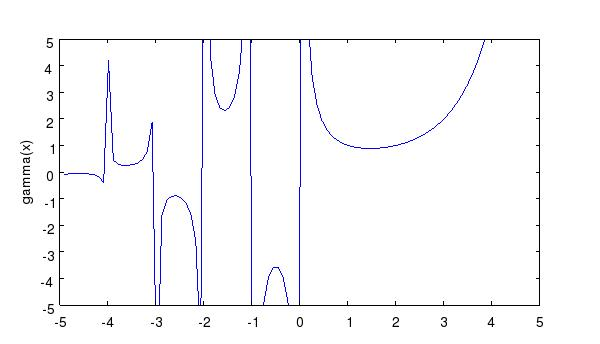
\includegraphics[width=8cm]{gamma1}}

